% set the problem in context.
% summarise what you have done.
% describe your design solution.
% report on its performance.
% provide key recommendations.
\section{Design}
The project aims to develop a solution to automate and thereby ease the beer production process for the hobbyists, our design solution is strictly developed based on the previously mentioned personas and requirements.\newline
This process can under normal circumstances be a rather complex and very manual process, the user would have to manually control the temperature, add the correct ingredients and the right amount at the right time, while continuously monitoring the process to ensure that everything is going according to plan.\newline
The user might want to produce both produce multiple amounts, but also different kinds of beer. This would require the user to look-up each recipe every time to do the same recipe calculations based on the desired amount and beer type with every new batch, while monitoring and possibly adjusting the temperatures of the ingredients throughout the whole process for consistency.\newline
This process can quickly become overwhelming and tedious, especially for newcomers, and might lead to human errors as the production expands and in worst case, end up taking the joy out of the hobby.\newline
Our design goal is to make brewing easy and accessible to everyone, even for the least technical of people. We want to solve this issue by having a simple and clean user interface, without all the unnecessary information, where all the heavy calculations, continuous monitoring, and processing is done by software behind the scenes.\newline
The design aims to deter people from the seemingly advanced process of beer production by offering an intuitive and easy-to-use platform that removes the complexity and makes brewing accessible to every intrigued hobbyist.

\subsection{System Architecture}
The architecture of the system is based on the client-server model and include three deployments: The web-service, the database service, and the physical beer machine. \newline
The Web Service will consist of the front-end, back-end, and the OPC Client. There will be a direct line of communication between the user input in the user interface, through the data processing and handling in the backend, to the OPC Client that will handle the secure communication and instructions to the physical beer machine. \newline
The communication between the front-end, the back-end and the beer machine is implemented using a RESTful API. \newline
This deployment model ensures a clear separation of concerns, enabling efficient scaling in the future, while easing the maintenance of individual components.

\subsection{Frontend}
The user interface (UI) of the beer production system is developed using React, a powerful and easy-to-use JavaScript library with a lot of flexibility and efficiency in building interactive and dynamic user interfaces, which perfectly aligned with our goal of creating a user-friendly and responsive frontend for the beer production application.
In addition, Reacts offers a modular development environment in form of it's component-based design structure, this allows for the development of reusable UI elements, that can be combined to effortlessly form complex user interfaces. This helped the project to meet requirement U-01, to develop a user-friendly design, as each component can be developed and tested individually, before it's combined to form the final UI. \newline
The library also offers a virtual DOM (Document Object Model), which is a lightweight representation of the actual DOM, this allows for efficient rendering of the UI, as the virtual DOM only updates the necessary components, instead of re-rendering the whole UI every time a change is made. This helped the project to meet requirement U-02, to develop a responsive design, as the virtual DOM allows for efficient rendering of the UI, which in turn allows for a more responsive UI. \newline
Lastly it offered us a lot of flexibility in terms of state management, which is a crucial aspect of the project, as the UI needs to be able to handle a lot of different states, such as the different stages of the beer production process, and the different states of the beer machine. This helped the project to meet requirement U-03, to develop a dynamic design, as the UI can be updated to reflect the current state of the beer machine and it's progress. \newline
All these features, combined with the fact that it is a very popular and well-documented library, made it the perfect choice for the development of the user interface of the beer production system.
\subsubsection{User Interface}
To ensure we met requirement U-01, to develop a user-friendly design, we decided to develop a clean and simple user interface, without all the unnecessary information, to make it as easy as possible for the user to navigate and use the application. \newline
Therefore, an early draft of the user interface was developed to get a clear idea of the overall design and layout of the application. \newline
\begin{center}
  \centering
  \begin{figure}[H]
      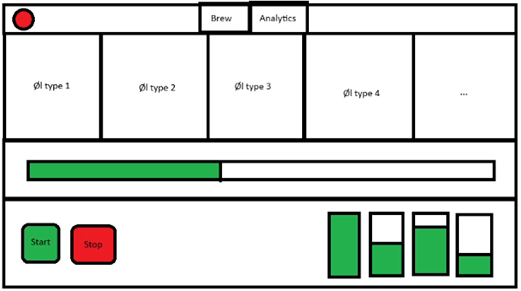
\includegraphics[width=1\textwidth]{img/frontend-draft.png}
      \caption{Early draft of the user interface}
      \label{fig:Frontend_draft}
  \end{figure}
\end{center}
With attention to the user experience, the user interface was designed to be intuitive and easy to use, with a clear and simple layout, and a minimalistic design. \newline
At the top of the page, the user is presented with 2 tabs: the \textit{Brew} tab and the \textit{Analytic} tab.  \newline
The \textit{Brew} tab is the default tab, and this is where the user can initiate the beer production process. \newline
The user is at the top presented with a column of the available beer types, and the user can select the desired beer type by clicking on the corresponding button. \newline
Below the beer type buttons a progress bar is displayed, this progress bar will be updated to reflect the current stage of the beer production process. \newline
At the bottom of the page, the column is divided into 2 sections: the left section contains \textit{Control buttons} to either start or stop the production, and the right side contains the \textit{Silo fill level} which visually indicates the current level of material stored in the silo. \newline
To brew a beer, the user simply selects the desired beer type, followed by pressing the big green \textit{Start} button at the bottom left.

\subsection{Backend}
The backend component of the beer production system will be implemented using Node.js, a versatile JavaScript runtime known for its efficiency in building scalable and high-performance server-side applications. Leveraging the strengths of Node.js, we aim to create a secure and reliable back-end that seamlessly communicates with the front end and the PLC-controlled beer production machine.
Node was chosen over Milo, for various reasons. Firstly, Node is a more well-documented framework it runs on the newest version of Java, which makes it easier to find solutions to problems and to get help when needed. Secondly, Node is a more versatile framework, which allows for more flexibility in terms of development. Lastly, Node is a more popular framework, which means that it has a larger community, which in turn means that it is more likely to be supported in the future. \newline
This design choice also enabled us to easily implement and use the OPCUA library, as it allows us to easily implement a secure communication with the beer machine by automatically generating the certificate needed for communication. \newline

\subsection{communication}
The communication between the front-end and the back-end is implemented using a RESTful API. 

\subsection{Simulation}
Incorporating the provided ARsim simulation tool early on into our development process was a crucial aspect of this project in terms of testing. 
The early integration allowed us to speed up the development time from the very beginning, as most of our program's functionalities could be tested directly without the need for direct access to the physical machine.
The tool allowed us to interact with ARsim in a manner similar to how our software would communicate with the actual machine, but it also enabled multiple people to test multiple different things without interfering with one another.
% ARsim serves as a valuable resource that enables simulation of the beer production process without the need for direct access to the physical machine. 
%This simulation tool will be instrumental in testing and refining our software application.

\subsubsection{ARsim Integration}
The ARsim simulation tool was integrated early into the development process, to mimic the behavior of the beer machine.
The early integration allowed us to speed up the development time from the very beginning of the project, as most of our program's functionalities could be tested directly without the need of the physical beer machine.
This integration also allowed us to interact with ARsim in a manner similar to how our software would communicate with the actual hardware, and enabled multiple people to test multiple different things without interfering with one another. 
% By leveraging ARsim, we can perform comprehensive testing of the software's functionalities, ensuring robustness and reliability.

\subsubsection{Testing Scenarios}


\subsection{Data Processing and Logging}

\subsection{Security Measures}

\subsection{Prioritization of Requirements}

\subsection*{Development Methodology}

\subsection*{Risk and Mitigation}

\subsection{Project Organization}

\subsection{Deliverables}